% Apresentação de Defesa de TCC - Daniel Cavalli
% Instituto de Economia - UFRJ
% 2025 - Versão Clean/Minimalista

\documentclass[10pt,aspectratio=169]{beamer}

% Pacotes essenciais
\usepackage[brazilian]{babel}
\usepackage[utf8]{inputenc}
\usepackage[T1]{fontenc}
\usepackage{amsmath,amssymb}
\usepackage{graphicx}
\usepackage{booktabs}
\usepackage{multirow}
\usepackage{tikz}
\usepackage{pgfplots}
\pgfplotsset{compat=1.17}

% Tema minimalista personalizado
\usetheme{default}
\useinnertheme{rectangles}
\useoutertheme{infolines}
\usecolortheme{default}

% Remove todos os elementos decorativos
\setbeamertemplate{navigation symbols}{}
\setbeamertemplate{blocks}[default]
\setbeamertemplate{title page}[default][colsep=-4bp,rounded=false]
\setbeamertemplate{part page}[default][colsep=-4bp,rounded=false]
\setbeamertemplate{itemize items}[circle]
\setbeamertemplate{enumerate items}[default]

% Cores UFRJ minimalistas
\definecolor{ufrjblue}{RGB}{0,53,96}
\definecolor{ufrjlightgray}{RGB}{245,245,245}
\definecolor{ufrjdarkgray}{RGB}{80,80,80}
\definecolor{ufrjaccent}{RGB}{51,102,153}

% Esquema de cores limpo
\setbeamercolor{structure}{fg=ufrjblue}
\setbeamercolor{title}{fg=ufrjblue}
\setbeamercolor{frametitle}{fg=ufrjblue,bg=white}
\setbeamercolor{normal text}{fg=ufrjdarkgray,bg=white}
\setbeamercolor{alerted text}{fg=red!80!black}
\setbeamercolor{example text}{fg=green!50!black}

% Blocos minimalistas
\setbeamercolor{block title}{fg=white,bg=ufrjblue}
\setbeamercolor{block body}{fg=black,bg=ufrjlightgray}
\setbeamercolor{block title alerted}{fg=white,bg=red!80!black}
\setbeamercolor{block body alerted}{fg=black,bg=red!10}
\setbeamercolor{block title example}{fg=white,bg=green!50!black}
\setbeamercolor{block body example}{fg=black,bg=green!10}

% Itens
\setbeamercolor{itemize item}{fg=ufrjblue}
\setbeamercolor{itemize subitem}{fg=ufrjaccent}
\setbeamercolor{enumerate item}{fg=ufrjblue}

% Rodapé minimalista
\setbeamertemplate{footline}{
  \hbox{%
  \begin{beamercolorbox}[wd=.5\paperwidth,ht=2.5ex,dp=1.125ex,leftskip=.3cm,rightskip=.3cm]{author in head/foot}%
    \usebeamerfont{author in head/foot}\insertshortauthor \hfill \insertshorttitle
  \end{beamercolorbox}%
  \begin{beamercolorbox}[wd=.5\paperwidth,ht=2.5ex,dp=1.125ex,leftskip=.3cm,rightskip=.3cm plus1fil]{title in head/foot}%
    \usebeamerfont{title in head/foot}\hfill\insertframenumber\,/\,\inserttotalframenumber
  \end{beamercolorbox}}%
  \vskip0pt%
}

% Fontes
\usefonttheme{professionalfonts}
\setbeamerfont{title}{size=\LARGE,series=\bfseries}
\setbeamerfont{subtitle}{size=\large,series=\mdseries}
\setbeamerfont{frametitle}{size=\Large,series=\bfseries}
\setbeamerfont{framesubtitle}{size=\large,series=\mdseries}
\setbeamerfont{block title}{size=\normalsize,series=\bfseries}
\setbeamerfont{footline}{size=\tiny}

% Espaçamentos
\setbeamersize{text margin left=1.5em,text margin right=1.5em}

% Remove sombras de todas as caixas
\makeatletter
\def\beamer@shadowbox#1#2#3#4{%
  \setbox\beamer@tempbox=\hbox{{#4}}%
  \hskip-#1%
  \vbox{%
    \vskip-#2%
    \box\beamer@tempbox}}
\makeatother

% Informações do documento
\title[Estações Meteorológicas e Produtividade]{Impacto de Estações Meteorológicas na\\Produtividade Agrícola}
\subtitle{Uma Aplicação de Diferenças em Diferenças\\com Tratamento Escalonado}
\author[Daniel Cavalli]{Daniel Cavalli}
\institute[IE-UFRJ]{
  Instituto de Economia -- UFRJ\\[0.3cm]
  \small Orientador: Prof. Romero Rocha
}
\date{2025}

% Importa valores automaticamente gerados
% Arquivo gerado automaticamente por generate_latex_values.r
% Última atualização: 2025-09-07

% Valores do teste placebo aleatório
\newcommand{\placebotruatt}{0.082}
\newcommand{\placebopvalue}{< 0,001}
\newcommand{\placebolower}{-0.037}
\newcommand{\placeboupper}{0.033}
\newcommand{\placebonsims}{50}
\newcommand{\placebomean}{-0.002}

% Valores formatados para texto
\newcommand{\placebotruattpct}{8.2\%}
\newcommand{\placebopvaluepct}{< 1\%}

% Valores do modelo principal
\newcommand{\mainatt}{0.082}
\newcommand{\mainse}{0.032}
\newcommand{\mainattpct}{8.2\%}

% Valores da análise de sensibilidade temporal
% Completo (2003-2023)
\newcommand{\sensfullatt}{0.126}
\newcommand{\sensfullse}{0.029}
\newcommand{\sensfulllower}{0.070}
\newcommand{\sensfullupper}{0.182}
\newcommand{\sensfulln}{7371}
% Excluindo Início (2006-2023)
\newcommand{\sensnostartatt}{0.130}
\newcommand{\sensnostartse}{0.031}
\newcommand{\sensnostartlower}{0.069}
\newcommand{\sensnostartupper}{0.191}
\newcommand{\sensnostartn}{6318}
% Excluindo Final (2003-2019)
\newcommand{\sensnoendatt}{0.117}
\newcommand{\sensnoendse}{0.027}
\newcommand{\sensnoendlower}{0.065}
\newcommand{\sensnoendupper}{0.170}
\newcommand{\sensnoendn}{5967}
% Excluindo COVID (2003-2019)
\newcommand{\sensnocovidatt}{0.117}
\newcommand{\sensnocovidse}{0.026}
\newcommand{\sensnocovidlower}{0.066}
\newcommand{\sensnocovidupper}{0.169}
\newcommand{\sensnocovidn}{5967}
% Pré-COVID (2003-2019)
\newcommand{\sensprecovidatt}{0.117}
\newcommand{\sensprecovidse}{0.025}
\newcommand{\sensprecovidlower}{0.068}
\newcommand{\sensprecovidupper}{0.167}
\newcommand{\sensprecovidn}{5967}


% Início do documento
\begin{document}

% Slide título customizado
\begin{frame}[plain]
\begin{tikzpicture}[remember picture,overlay]
    \fill[ufrjblue] (current page.north west) rectangle ([yshift=-3cm]current page.north east);
\end{tikzpicture}
\vspace{1cm}
{\color{white}\Large\bfseries\inserttitle}\\[0.5cm]
{\color{white}\large\insertsubtitle}\\[1cm]
{\large\insertauthor}\\[0.3cm]
{\small\insertinstitute}\\[0.5cm]
{\small\insertdate}
\end{frame}

% Sumário
\begin{frame}{Sumário}
\tableofcontents
\end{frame}

% ===== SEÇÃO 1: INTRODUÇÃO =====
\section{Introdução}

\begin{frame}{Motivação}
\begin{itemize}
    \item A agricultura brasileira enfrenta o desafio de aumentar a produtividade em contexto de crescente variabilidade climática
    \vspace{0.3cm}
    \item Informação meteorológica precisa emerge como insumo produtivo crítico
    \vspace{0.3cm}
    \item \textbf{Lacuna na literatura}: ausência de evidências causais sobre o impacto econômico da expansão da infraestrutura meteorológica
    \vspace{0.3cm}
    \item Instalação escalonada de estações (2000-2019) oferece experimento natural
\end{itemize}

\begin{block}{Questão Central}
Qual é o impacto causal da instalação de estações meteorológicas sobre o PIB agropecuário?
\end{block}
\end{frame}

\begin{frame}{Objetivos}
\begin{columns}
\column{0.5\textwidth}
\textbf{Objetivo Geral:}
\begin{itemize}
    \item Estimar o efeito causal da instalação de estações meteorológicas sobre a produtividade agrícola
\end{itemize}

\column{0.5\textwidth}
\textbf{Objetivos Específicos:}
\begin{enumerate}
    \item Aplicar metodologia adequada para tratamento escalonado
    \item Quantificar o retorno econômico da infraestrutura
    \item Analisar a dinâmica temporal dos efeitos
    \item Validar robustez dos resultados
\end{enumerate}
\end{columns}

\vspace{0.5cm}
\begin{alertblock}{Contribuição Principal}
Primeira evidência causal rigorosa do impacto econômico de estações meteorológicas na agricultura brasileira
\end{alertblock}
\end{frame}

% ===== SEÇÃO 2: REVISÃO DA LITERATURA =====
\section{Revisão da Literatura}

\begin{frame}{Canais de Impacto da Informação Meteorológica}
\begin{columns}
\column{0.5\textwidth}
\textbf{Literatura Internacional:}
\begin{itemize}
    \item \textbf{Mavi \& Tupper (2004)}: três dimensões de impacto
    \begin{itemize}
        \item Planejamento estratégico
        \item Decisões táticas
        \item Resiliência sistêmica
    \end{itemize}
    \item \textbf{Weiss (2000)}: ajustes finos nas práticas
    \item \textbf{Rijks (2000)}: ganhos econômicos potenciais
\end{itemize}

\column{0.5\textwidth}
\textbf{Contexto Brasileiro:}
\begin{itemize}
    \item \textbf{Monteiro (2009)}: oscilações meteorológicas determinam produção
    \item \textbf{Carvalho et al. (2015)}: impacto climático na cana-de-açúcar
    \item \textbf{Vianna \& Sentelhas (2016)}: otimização via modelos agrometeorológicos
\end{itemize}
\end{columns}

\vspace{0.3cm}
\begin{block}{Gap Identificado}
Estudos existentes são predominantemente descritivos ou baseados em correlações
\end{block}
\end{frame}

% ===== SEÇÃO 3: METODOLOGIA =====
\section{Metodologia}

\begin{frame}{O Problema do DiD Tradicional com Tratamento Escalonado}
\begin{columns}
\column{0.6\textwidth}
\textbf{Two-Way Fixed Effects (TWFE) tradicional:}
$$Y_{it} = \alpha_i + \lambda_t + \beta D_{it} + \epsilon_{it}$$

\textbf{Problemas identificados:}
\begin{itemize}
    \item Usa unidades já tratadas como controle
    \item Pesos negativos em algumas comparações
    \item Viés quando efeitos são heterogêneos
\end{itemize}

\column{0.4\textwidth}
\begin{figure}
\centering
\begin{tikzpicture}[scale=0.7]
\draw[->] (0,0) -- (5,0) node[right] {Tempo};
\draw[->] (0,0) -- (0,3) node[above] {Unidades};
\fill[blue!30] (1,0.5) rectangle (2,1);
\fill[blue!30] (2,1.5) rectangle (3,2);
\fill[blue!30] (3,2.5) rectangle (4,3);
\draw[red,thick] (1.5,1.5) -- (2.5,2) node[right,font=\tiny] {Comparação problemática};
\end{tikzpicture}
\caption*{Tratamento escalonado}
\end{figure}
\end{columns}

\vspace{0.3cm}
\begin{alertblock}{Solução}
Callaway \& Sant'Anna (2021): estimação separada por coorte e agregação apropriada
\end{alertblock}
\end{frame}

\begin{frame}{Metodologia de Callaway \& Sant'Anna (2021)}
\begin{enumerate}
    \item \textbf{Group-Time ATT}: Estima efeito para cada coorte $g$ no tempo $t$
    $$ATT(g,t) = E[Y_{it}(g) - Y_{it}(0) | G_i = g]$$
    
    \item \textbf{Agregação}: Combina ATT(g,t) com pesos apropriados
    $$\theta = \sum_{g} \sum_{t} w(g,t) \cdot ATT(g,t)$$
    
    \item \textbf{Estimadores}:
    \begin{itemize}
        \item Outcome Regression (OR)
        \item Inverse Probability Weighting (IPW)
        \item \textbf{Doubly Robust (DR)} $\checkmark$
    \end{itemize}
\end{enumerate}

\begin{block}{Pressuposto Central}
Tendências paralelas condicionais entre tratados e controles
\end{block}
\end{frame}

% ===== SEÇÃO 4: DADOS =====
\section{Dados}

\begin{frame}{Por que Cana-de-Açúcar?}
\begin{columns}
\column{0.5\textwidth}
\textbf{Relevância Econômica:}
\begin{itemize}
    \item 3º maior produtor mundial
    \item Presente em 490 microrregiões
    \item R\$ 52 bilhões em valor de produção (2023)
\end{itemize}

\textbf{Características Técnicas:}
\begin{itemize}
    \item Alta sensibilidade climática
    \item Ciclo produtivo longo (12-18 meses)
    \item Janelas críticas de plantio/colheita
\end{itemize}

\column{0.5\textwidth}
\textbf{Vantagens Metodológicas:}
\begin{itemize}
    \item Dados completos e confiáveis
    \item Produção contínua no período
    \item Distribuição geográfica ampla
    \item Variação temporal na adoção de estações
\end{itemize}

\begin{alertblock}{Implicação}
Cultura ideal para identificar impactos de informação meteorológica
\end{alertblock}
\end{columns}
\end{frame}

\begin{frame}{Construção do Dataset}
\begin{columns}
\column{0.5\textwidth}
\textbf{Fontes de Dados:}
\begin{itemize}
    \item INMET: 610 estações meteorológicas
    \item IBGE: PIB municipal e população
    \item PAM-IBGE: produção de cana-de-açúcar
    \item Período: 2003-2023
\end{itemize}

\textbf{Unidade de Análise:}
\begin{itemize}
    \item Microrregiões (490 produtoras)
    \item Agregação de dados municipais
    \item Painel balanceado: 10.290 obs
\end{itemize}

\column{0.5\textwidth}
\begin{figure}
\centering
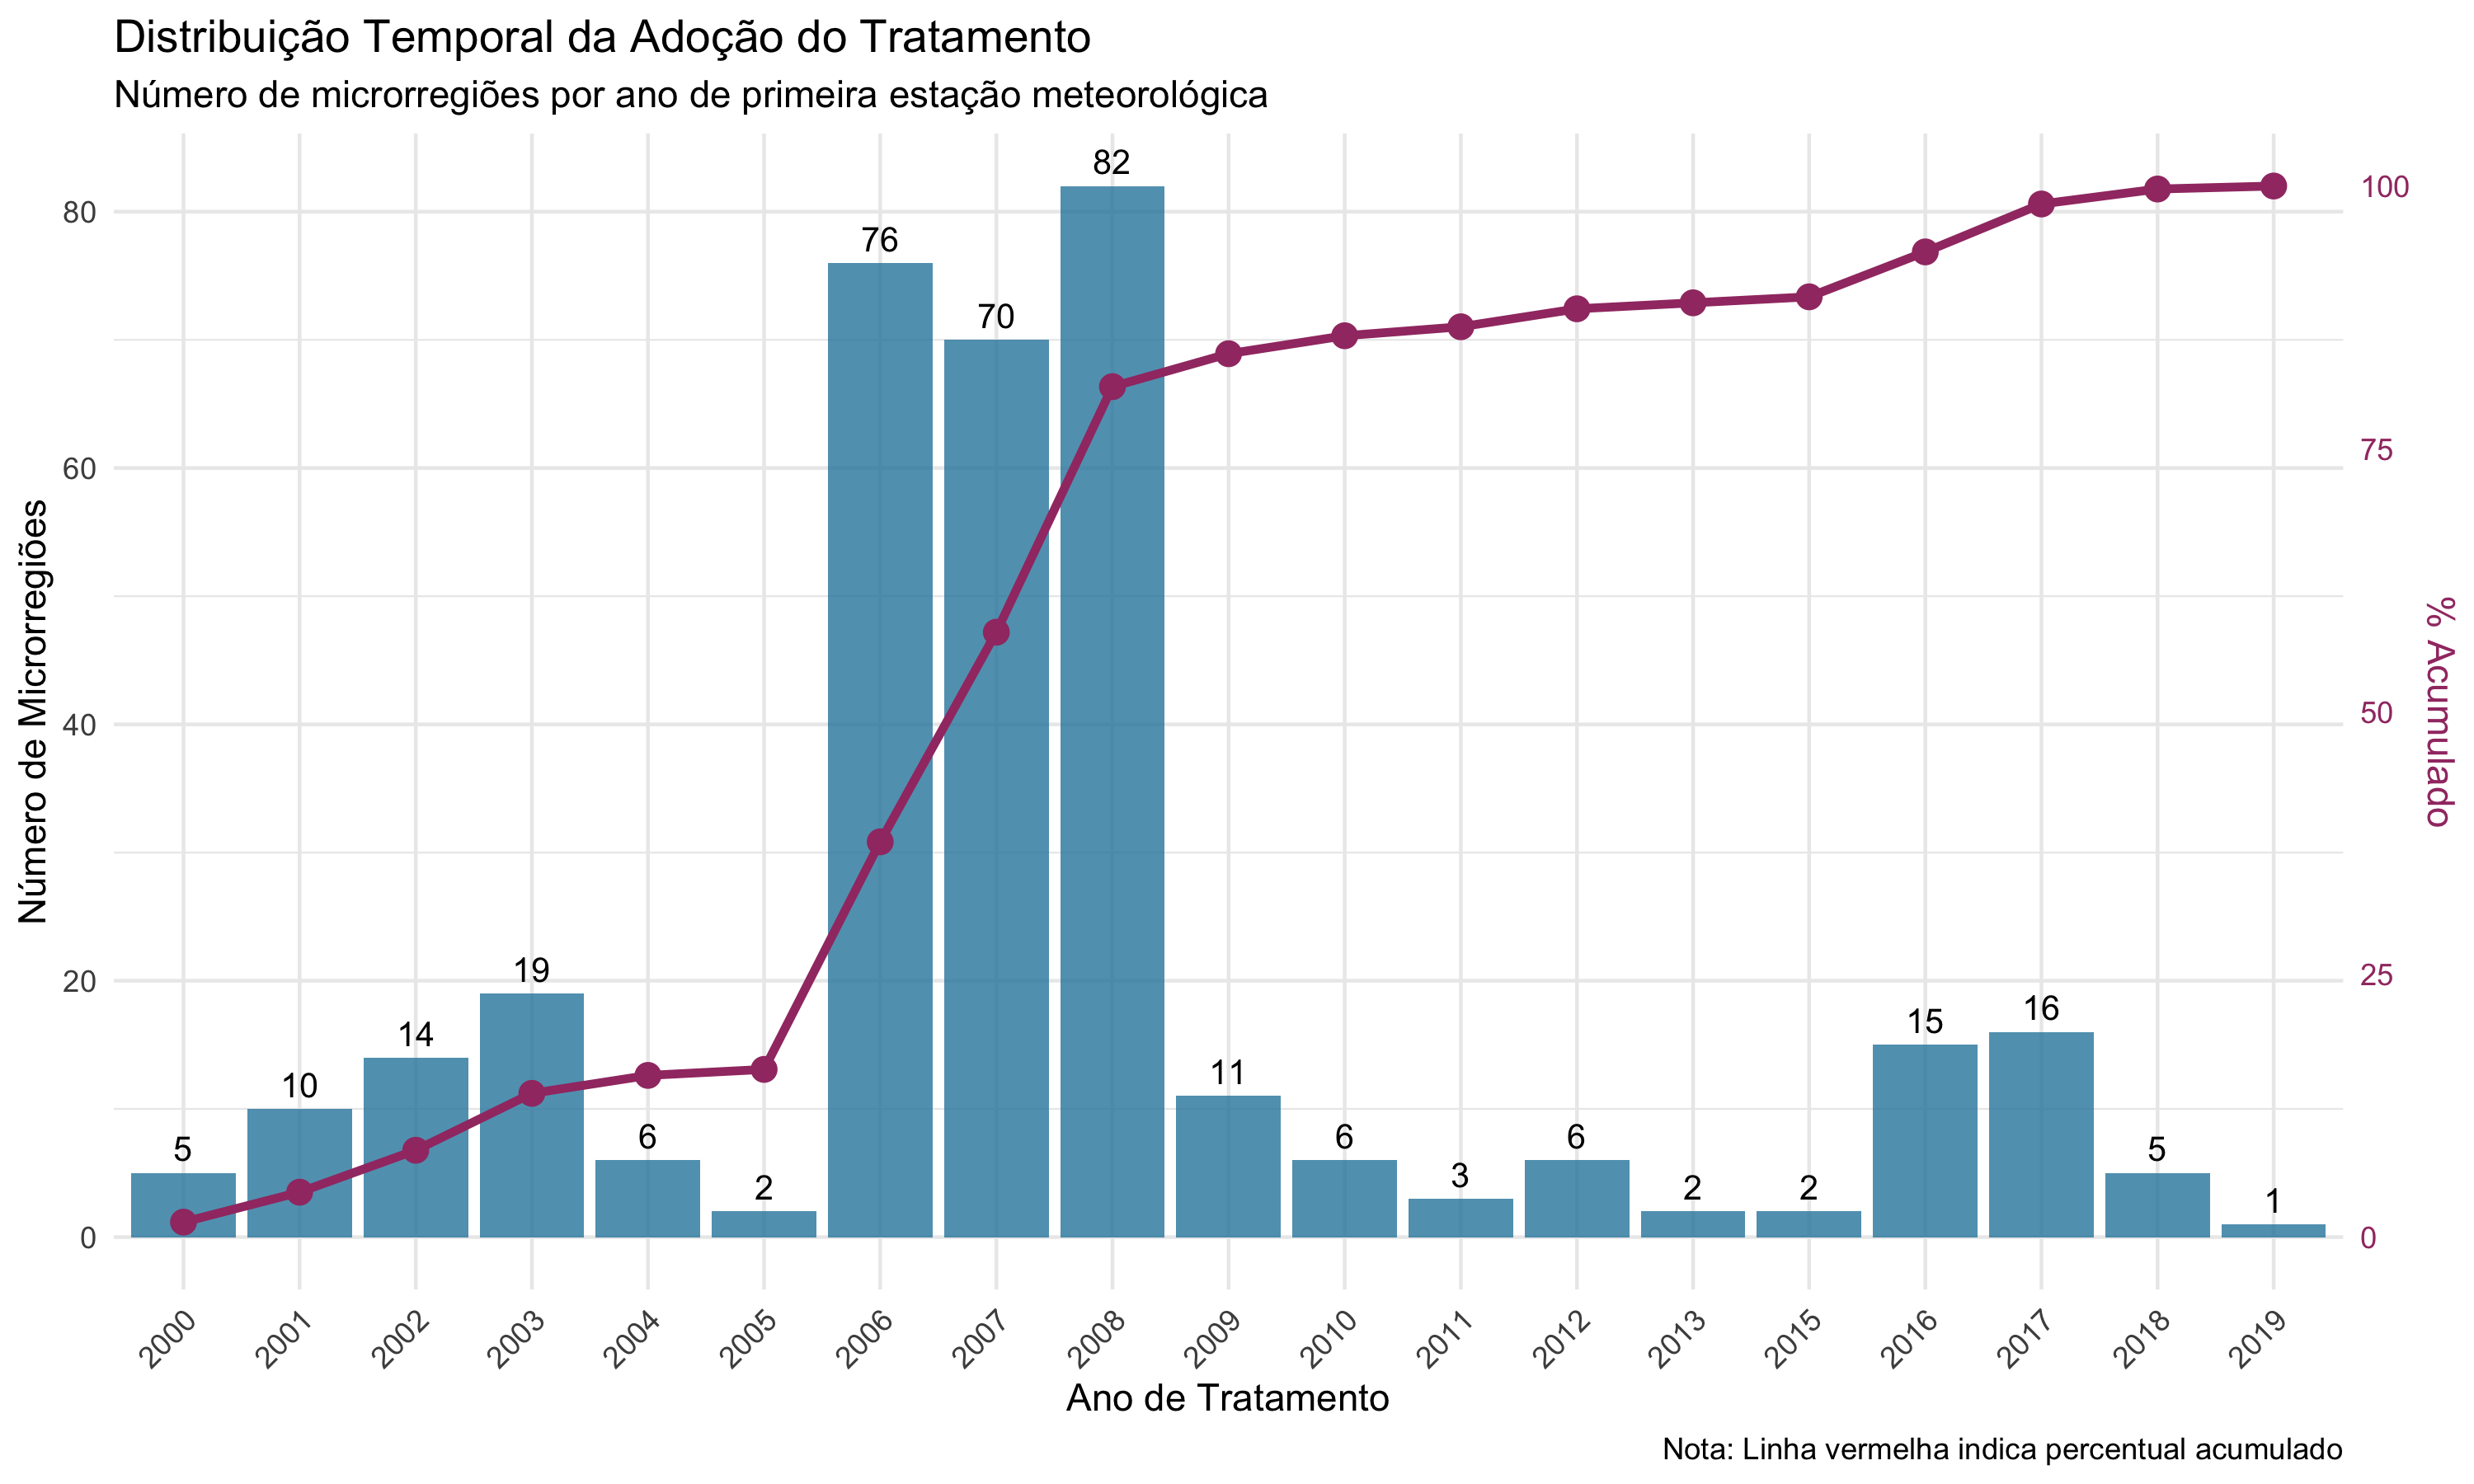
\includegraphics[width=\textwidth]{../../../data/outputs/descriptive_analysis/distribuicao_temporal_tratamento.png}
\caption{Distribuição Temporal do Tratamento}
\end{figure}
\end{columns}

\begin{block}{Transparência}
Código completo disponível em: \url{github.com/danielcavalli/tcc-ie-ufrj-2024}
\end{block}
\end{frame}

% ===== SEÇÃO 5: RESULTADOS =====
\section{Resultados}

\begin{frame}{Resultado Principal}
\begin{center}
\Large
\textbf{ATT = \mainatt{} (8,2\%)}\\
\normalsize
EP = \mainse, p = 0,0103\\
IC 95\%: [0,0194; 0,1448]
\end{center}

\begin{columns}
\column{0.5\textwidth}
\begin{table}[h]
\centering
\small
\begin{tabular}{lcc}
\toprule
Especificação & ATT & P-valor \\
\midrule
\textbf{Doubly Robust} & \textbf{0,082} & \textbf{0,010} \\
IPW & 0,094 & 0,003 \\
Regression & 0,066 & 0,030 \\
Sem covariáveis & 0,110 & 0,000 \\
\midrule
Never-treated & 0,080 & 0,026 \\
\bottomrule
\end{tabular}
\end{table}

\column{0.5\textwidth}
\textbf{Interpretação:}
\begin{itemize}
    \item Aumento de 8,2\% no PIB agropecuário
    \item Equivalente a 2+ anos de crescimento típico
    \item Robusto a diferentes especificações
    \item Economicamente significativo
\end{itemize}
\end{columns}

\begin{alertblock}{Implicação}
Retorno econômico supera amplamente os custos de instalação (R\$ 223 mil/estação)
\end{alertblock}
\end{frame}

\begin{frame}{Magnitude Econômica do Impacto}
\begin{columns}
\column{0.5\textwidth}
\textbf{Impacto por Microrregião:}
\begin{itemize}
    \item PIB agro médio: R\$ 580 milhões/ano
    \item Ganho de 8,2\%: R\$ 47,6 milhões/ano
    \item Payback: < 6 meses
\end{itemize}

\textbf{Projeção Nacional:}
\begin{itemize}
    \item 351 microrregiões tratadas
    \item Ganho agregado: R\$ 16,7 bilhões/ano
    \item 139 microrregiões sem estações
    \item Potencial não realizado: R\$ 6,6 bilhões/ano
\end{itemize}

\column{0.5\textwidth}
\begin{block}{Análise Custo-Benefício}
\begin{itemize}
    \item Custo médio por estação: R\$ 223 mil
    \item Retorno anual: R\$ 47,6 milhões
    \item Taxa de retorno: 213x ao ano
\end{itemize}
\end{block}

\begin{alertblock}{Conclusão}
Subinvestimento histórico representa oportunidade perdida de R\$ 6,6 bilhões anuais
\end{alertblock}
\end{columns}
\end{frame}

\begin{frame}{Event Study - Dinâmica Temporal}
\begin{figure}
\centering
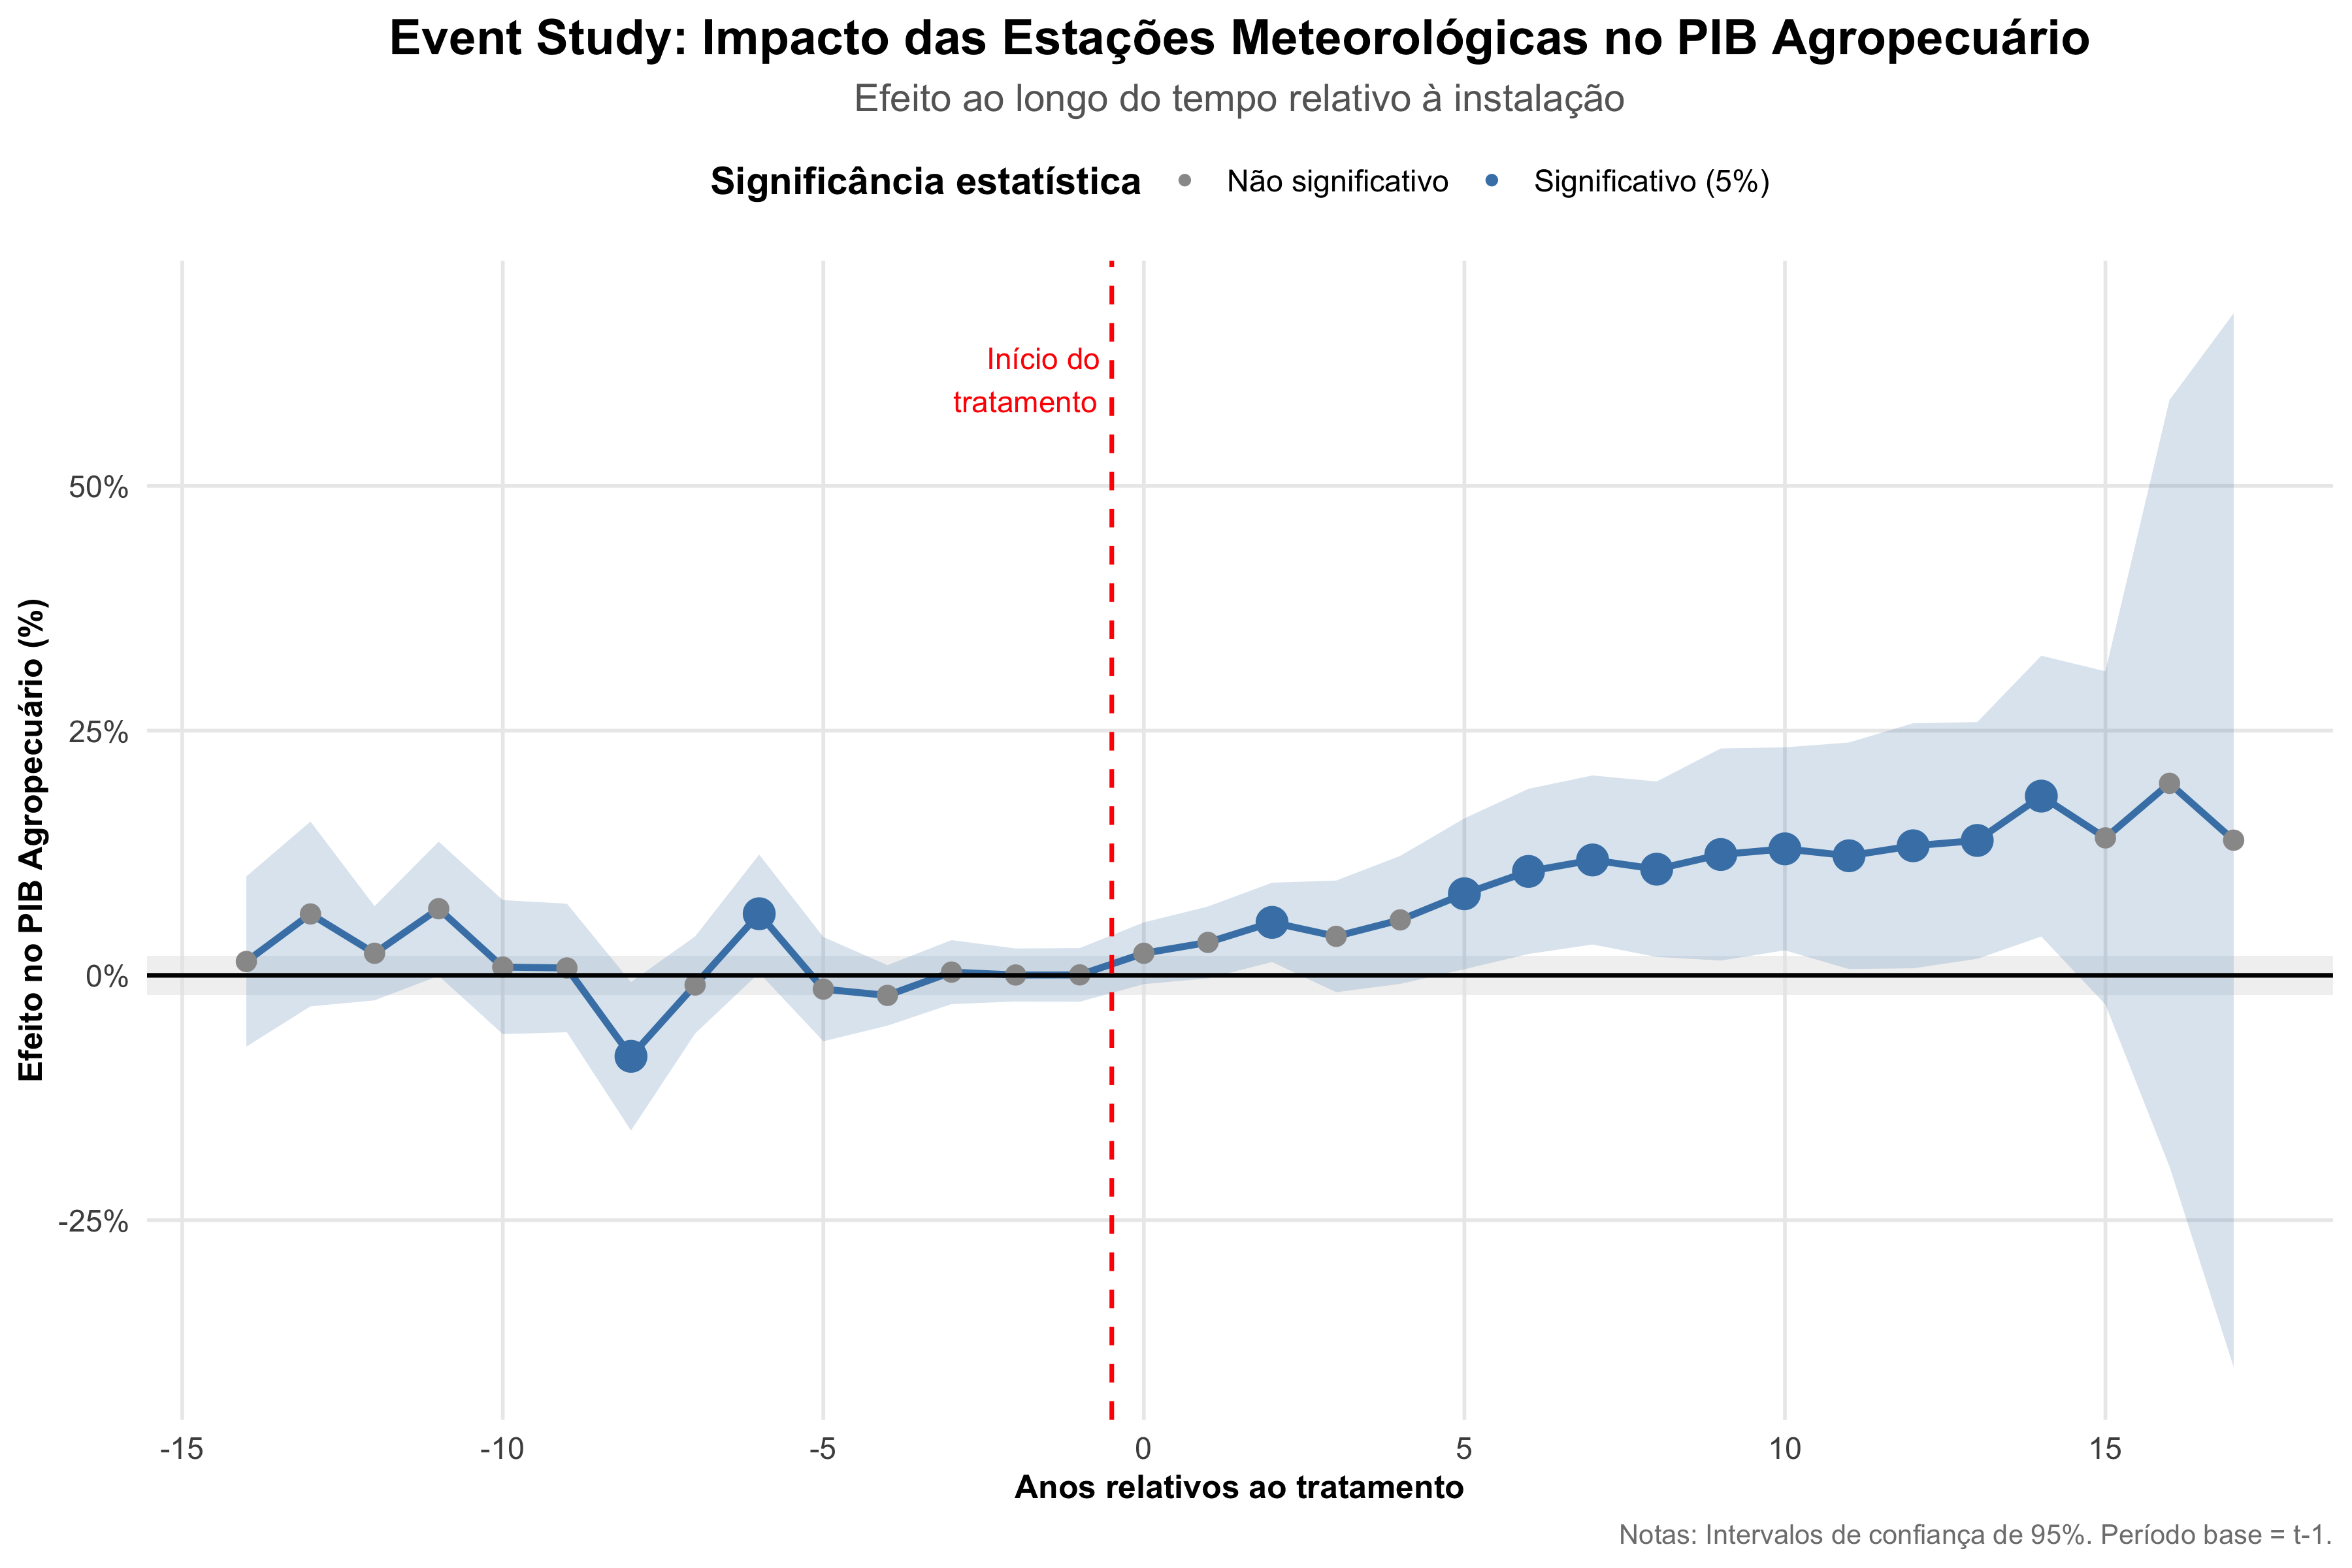
\includegraphics[width=0.85\textwidth]{../../../data/outputs/presentation/event_study_enhanced.png}
\end{figure}

\begin{columns}
\column{0.5\textwidth}
\textbf{Pré-tratamento:}
\begin{itemize}
    \item Ausência de tendências
    \item \textbf{Teste formal: F = 1,136 (p = 0,322)}
    \item Coeficientes oscilam aleatoriamente
    \item Forte evidência de parallel trends
\end{itemize}

\column{0.5\textwidth}
\textbf{Pós-tratamento:}
\begin{itemize}
    \item Efeitos positivos persistentes
    \item Difusão gradual dos benefícios
    \item Consistente com processo de aprendizado
    \item Estabilização em ~10\% após 5 anos
\end{itemize}
\end{columns}
\end{frame}

\begin{frame}{Tendências Paralelas - Validação Visual}
\begin{figure}
\centering
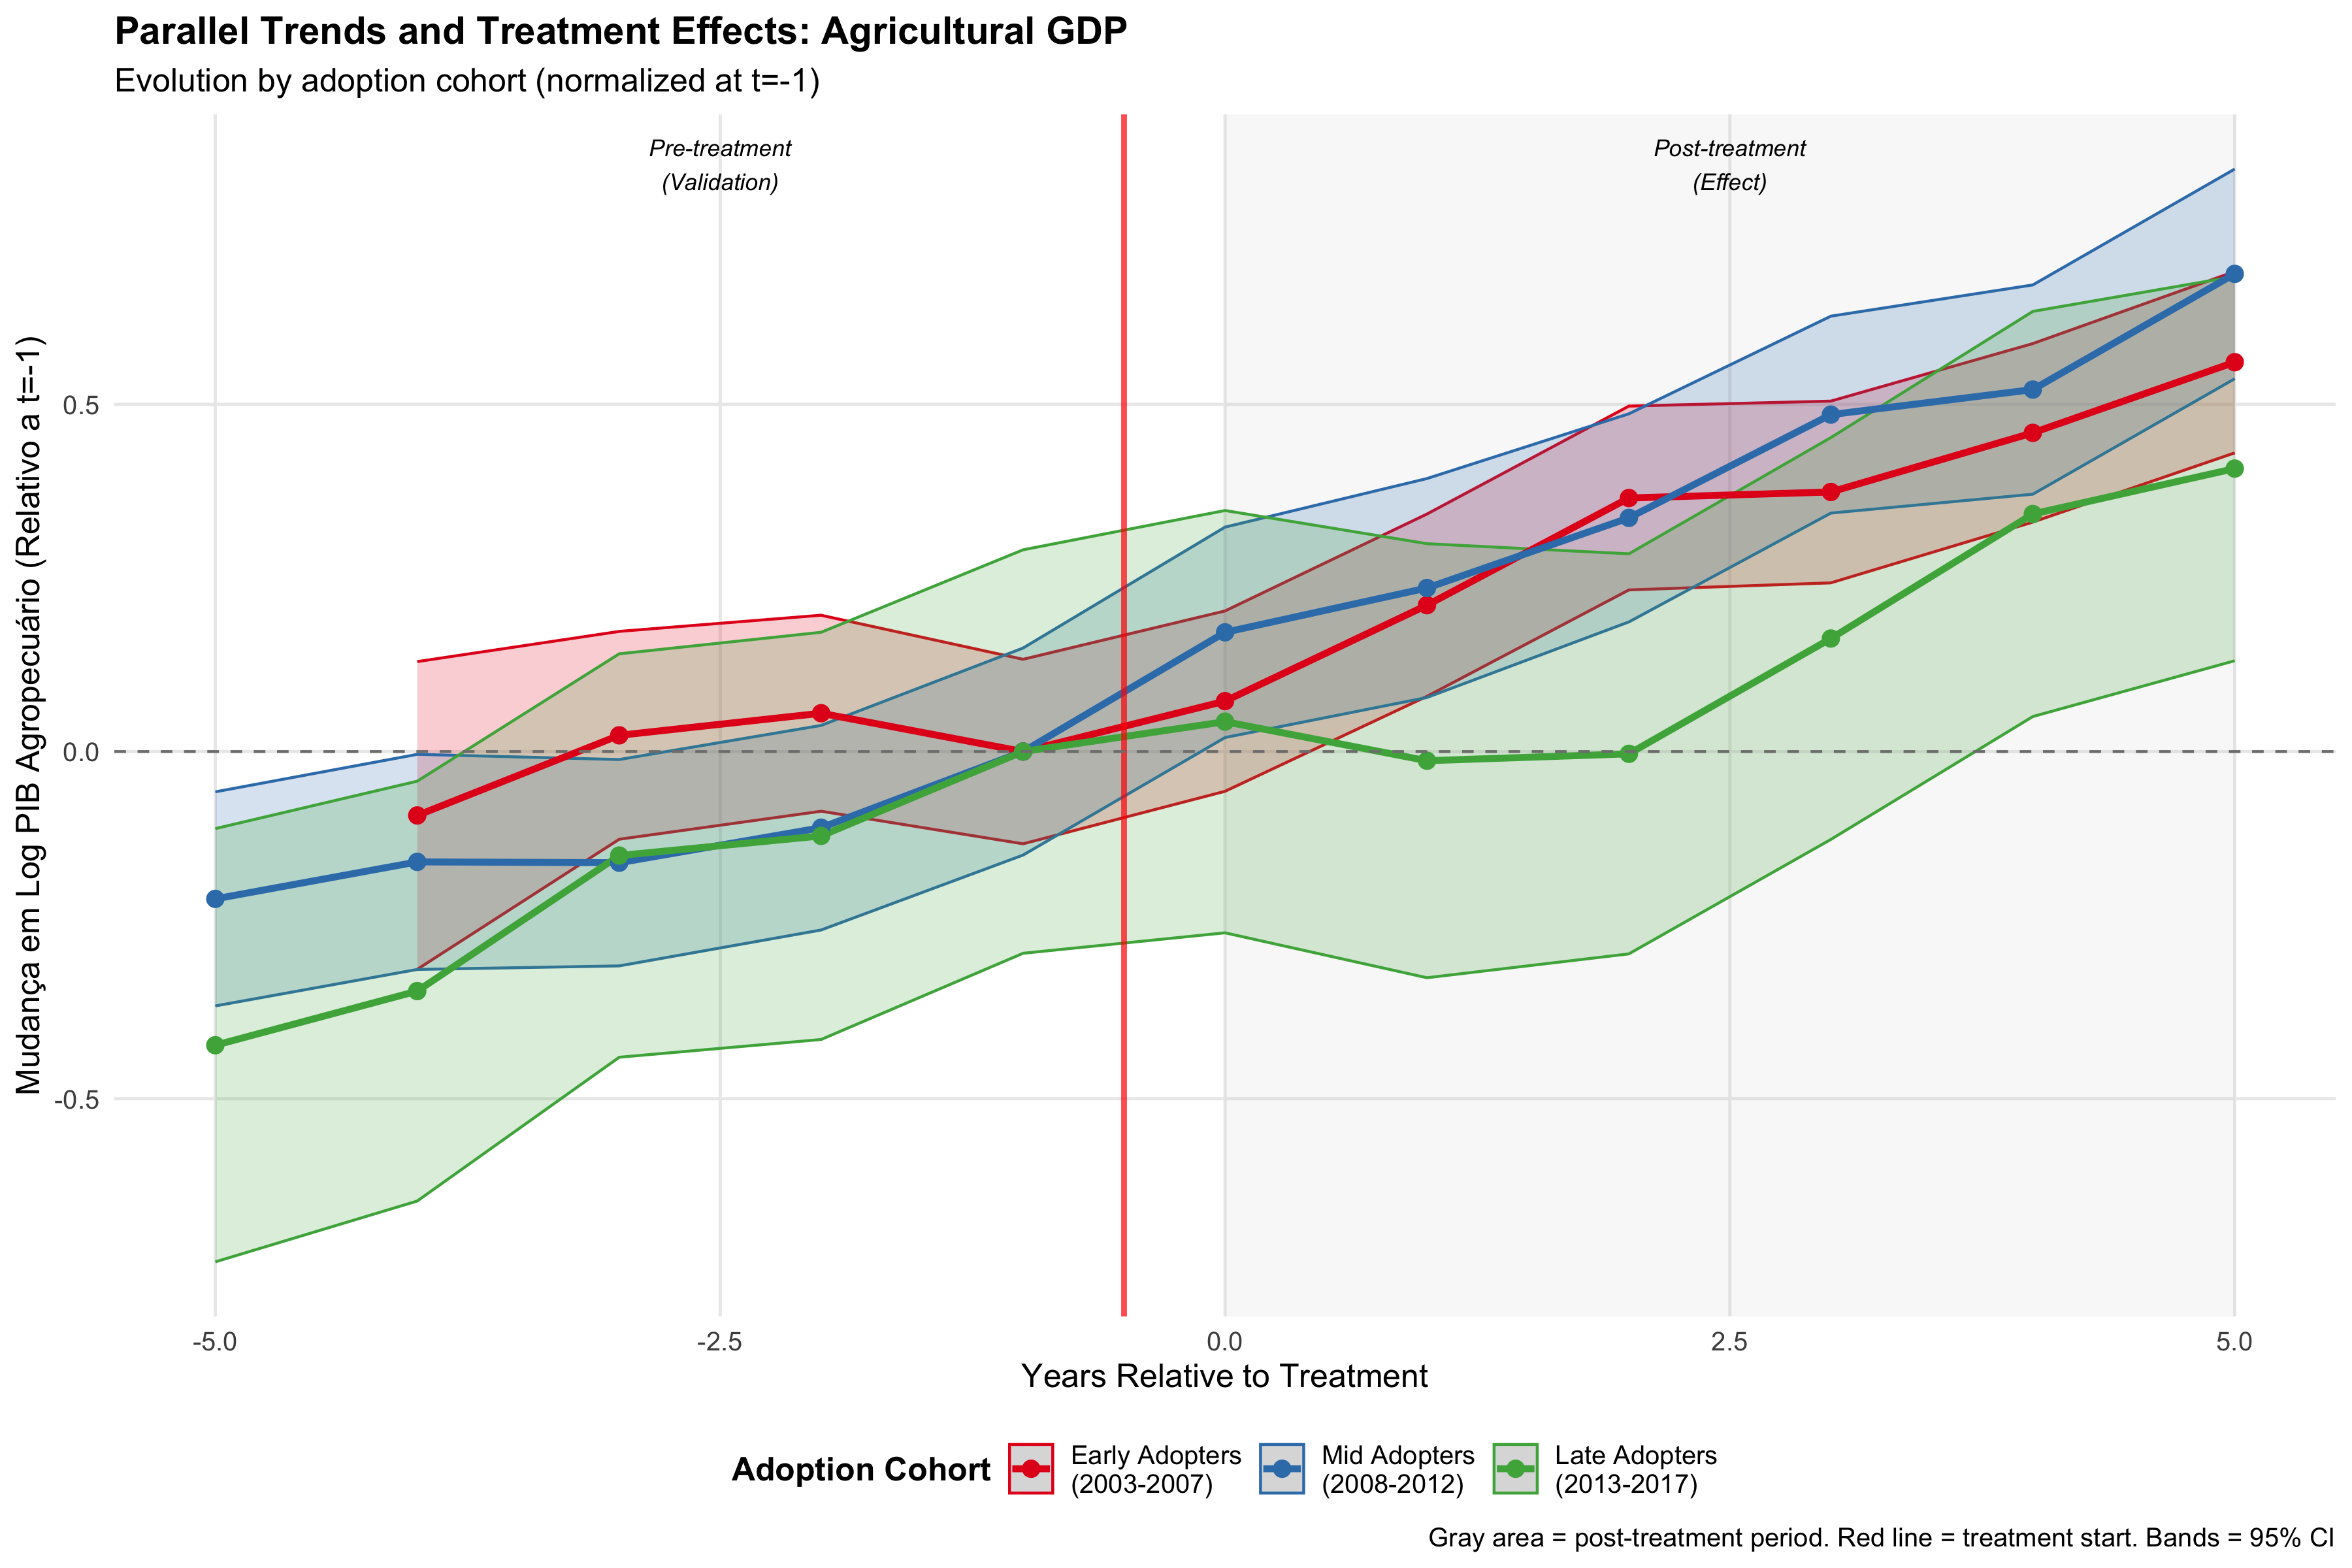
\includegraphics[width=0.8\textwidth]{../../../data/outputs/parallel_trends_complete_pib_agro_normalized.png}
\end{figure}

\begin{columns}
\column{0.5\textwidth}
\begin{itemize}
    \item Evolução similar pré-tratamento
    \item Divergência clara pós-instalação
    \item Sem antecipação do tratamento
\end{itemize}

\column{0.5\textwidth}
\begin{itemize}
    \item Grupos comparáveis
    \item Validação do pressuposto central
    \item Ganhos sustentados no tempo
\end{itemize}
\end{columns}
\end{frame}

% ===== SEÇÃO 6: ROBUSTEZ =====
\section{Análises de Robustez}

\begin{frame}{Teste Placebo - Randomização Múltipla}
\begin{figure}
\centering
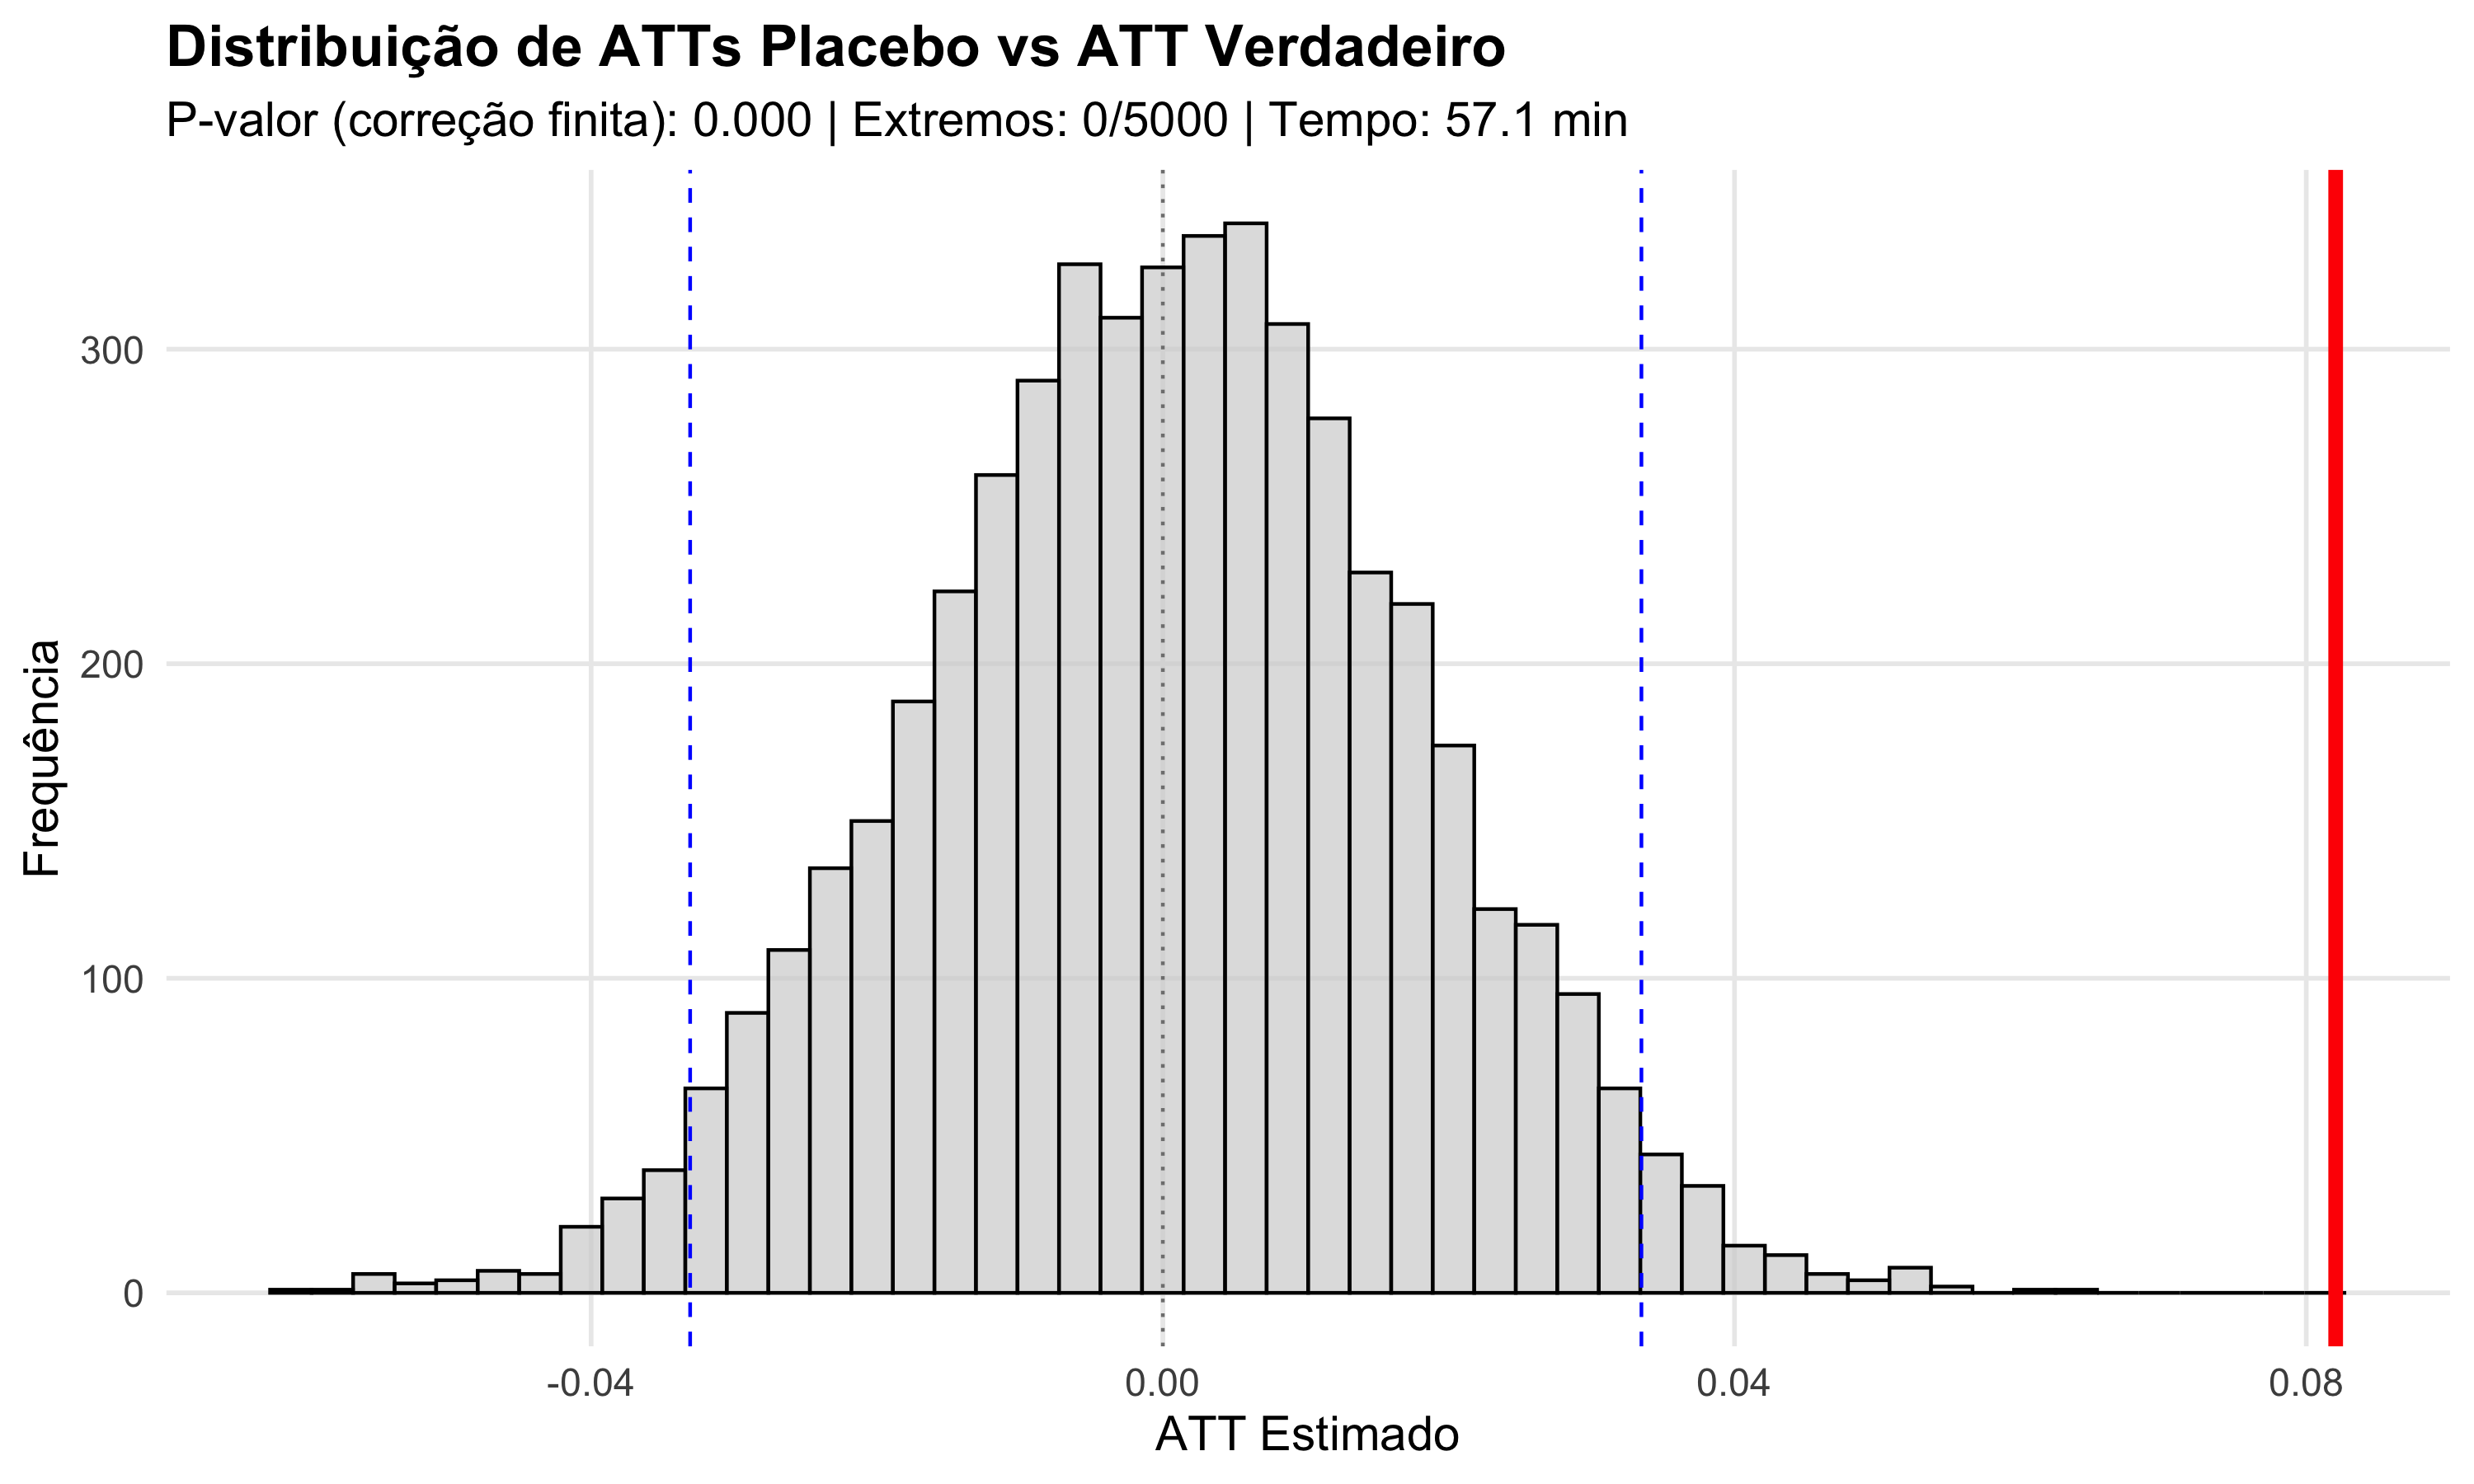
\includegraphics[width=0.7\textwidth]{../../../data/outputs/placebo_distribution.png}
\end{figure}

\begin{columns}
\column{0.5\textwidth}
\textbf{Metodologia:}
\begin{itemize}
    \item 50 simulações com tratamento aleatório
    \item Distribuição sob H0: sem efeito
    \item ATT verdadeiro vs. distribuição placebo
\end{itemize}

\column{0.5\textwidth}
\textbf{Resultados:}
\begin{itemize}
    \item Média placebo: \placebomean{}
    \item ATT verdadeiro: \placebotruatt{}
    \item P-valor empírico: \placebopvalue{}
    \item Menos de \placebopvaluepct{} por acaso
\end{itemize}
\end{columns}
\end{frame}

\begin{frame}{Análise de Robustez - Síntese}
\begin{figure}
\centering
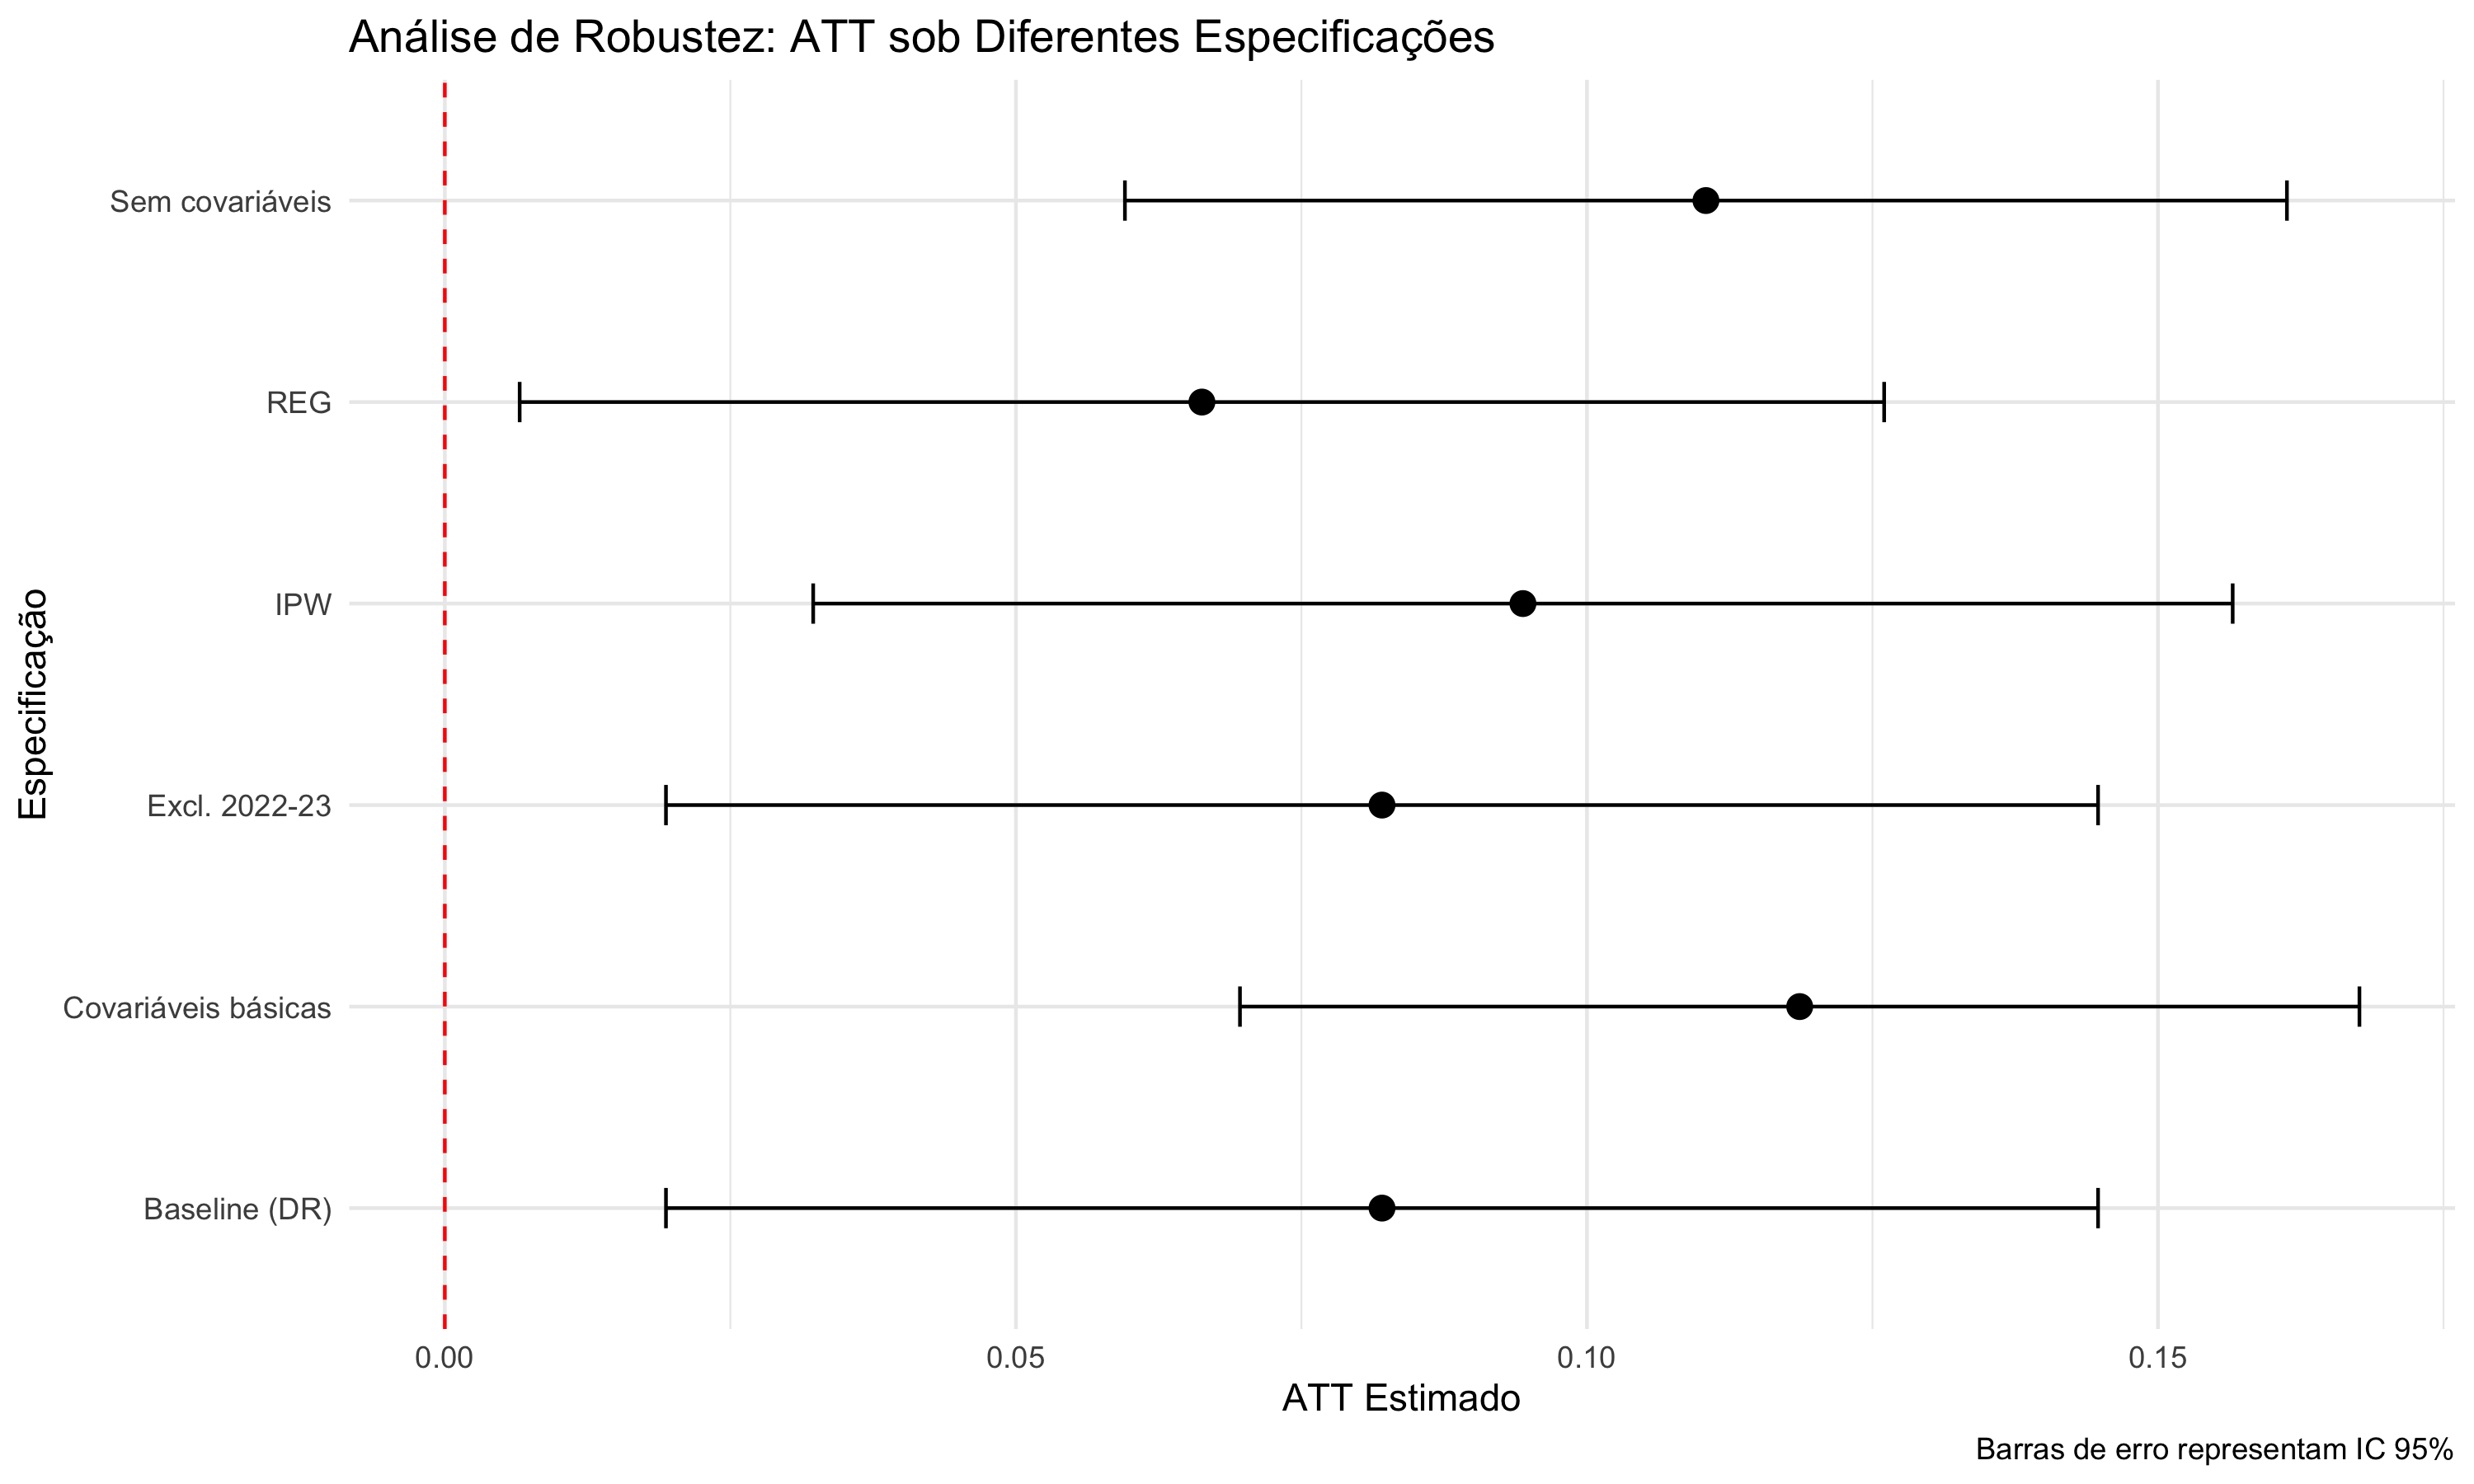
\includegraphics[width=0.9\textwidth]{../../../data/outputs/robustness_plot.png}
\end{figure}

\textbf{Testes Realizados:}
\begin{enumerate}
    \item Diferentes especificações econométricas (DR, IPW, REG)
    \item Grupos de controle alternativos (not-yet vs never-treated)
    \item Exclusão de períodos específicos (início, COVID)
    \item Placebo com PIB não-agropecuário: ATT = 0,030 (p = 0,365)
\end{enumerate}
\end{frame}

% ===== SEÇÃO 7: IMPLICAÇÕES =====
\section{Implicações para Políticas Públicas}

\begin{frame}{Contexto Atual e Recomendações}
\begin{columns}
\column{0.5\textwidth}
\textbf{Investimento Anunciado (Dez/2024):}
\begin{itemize}
    \item MAPA: R\$ 49 milhões
    \item 220 novas estações
    \item R\$ 223 mil/estação
\end{itemize}

\vspace{0.3cm}
\textbf{Nossos Resultados Sugerem:}
\begin{itemize}
    \item Retorno de 213x o investimento
    \item Payback < 6 meses
    \item Evidência empírica robusta
\end{itemize}

\column{0.5\textwidth}
\textbf{Recomendações:}
\begin{enumerate}
    \item \textbf{Expansão estratégica}
    \begin{itemize}
        \item Priorizar áreas não cobertas
        \item Foco em regiões produtoras
    \end{itemize}
    
    \item \textbf{Integração de dados}
    \begin{itemize}
        \item Sistemas como AGRITEMPO
        \item Acesso facilitado
    \end{itemize}
    
    \item \textbf{Capacitação}
    \begin{itemize}
        \item Uso efetivo das informações
        \item Assistência técnica
    \end{itemize}
\end{enumerate}
\end{columns}

\begin{block}{Urgência}
Atrasos na implementação representam perdas econômicas significativas
\end{block}
\end{frame}

% ===== SEÇÃO 8: LIMITAÇÕES =====
\section{Limitações e Pesquisa Futura}

\begin{frame}{Limitações do Estudo}
\begin{columns}
\column{0.5\textwidth}
\textbf{Limitações Identificadas:}
\begin{enumerate}
    \item \textbf{Desbalanceamento de covariáveis}
    \begin{itemize}
        \item Mitigado pelo DR
        \item Diferenças observáveis
    \end{itemize}
    
    \item \textbf{Composição dos pesos}
    \begin{itemize}
        \item Coortes iniciais: 50,8\%
        \item Sem dominância extrema
    \end{itemize}
    
    \item \textbf{Heterogeneidade não observada}
    \begin{itemize}
        \item Tamanho de propriedade
        \item Nível educacional
    \end{itemize}
\end{enumerate}

\column{0.5\textwidth}
\textbf{Direções Futuras:}
\begin{enumerate}
    \item \textbf{Modelagem espacial}
    \begin{itemize}
        \item Spillovers explícitos
        \item Dependência espacial
    \end{itemize}
    
    \item \textbf{Dados de alta frequência}
    \begin{itemize}
        \item Mensais/trimestrais
        \item Eventos climáticos
    \end{itemize}
    
    \item \textbf{Análise por cultura}
    \begin{itemize}
        \item Impactos diferenciados
        \item Outras culturas além da cana
    \end{itemize}
\end{enumerate}
\end{columns}

\begin{alertblock}{Apesar das Limitações}
Resultados robustos fornecem primeira evidência causal rigorosa
\end{alertblock}
\end{frame}

% ===== SEÇÃO 9: CONCLUSÕES =====
\section{Conclusões}

\begin{frame}{Conclusões Principais}
\begin{enumerate}
    \item \textbf{Evidência Causal Pioneira}
    \begin{itemize}
        \item Primeira quantificação rigorosa do impacto
        \item ATT = 8,2\% (p = 0,010)
        \item Efeito economicamente significativo
    \end{itemize}
    
    \item \textbf{Validação Metodológica}
    \begin{itemize}
        \item Superioridade do DiD escalonado
        \item Importância de métodos adequados
        \item Modelo para futuras aplicações
    \end{itemize}
    
    \item \textbf{Implicações Práticas}
    \begin{itemize}
        \item Justifica expansão da rede
        \item Alternativa à expansão da fronteira agrícola
        \item Estratégia de adaptação climática
    \end{itemize}
\end{enumerate}

\begin{block}{Mensagem Final}
Investimento em informação meteorológica é estratégia custo-efetiva para aumentar produtividade agrícola sustentavelmente
\end{block}
\end{frame}

% ===== REFERÊNCIAS =====
\begin{frame}[allowframebreaks]{Referências Principais}
\footnotesize
\begin{itemize}
    \item CALLAWAY, B.; SANT'ANNA, P. H. Difference-in-differences with multiple time periods. \textit{Journal of Econometrics}, v. 225, n. 2, p. 200-230, 2021.
    
    \item GOODMAN-BACON, A. Difference-in-differences with variation in treatment timing. \textit{Journal of Econometrics}, v. 225, n. 2, p. 254-277, 2021.
    
    \item MAVI, H. S.; TUPPER, G. J. \textit{Agrometeorology: principles and applications of climate studies in agriculture}. CRC Press, 2004.
    
    \item MONTEIRO, J. E. (Ed.). \textit{Agrometeorologia dos cultivos: o fator meteorológico na produção agrícola}. Brasília: INMET, 2009.
    
    \item SANT'ANNA, P. H.; ZHAO, J. Doubly robust difference-in-differences estimators. \textit{Journal of Econometrics}, v. 219, n. 1, p. 101-122, 2020.
    
    \item SUN, L.; ABRAHAM, S. Estimating dynamic treatment effects in event studies with heterogeneous treatment effects. \textit{Journal of Econometrics}, v. 225, n. 2, p. 175-199, 2021.
\end{itemize}
\end{frame}

% Slide final
\begin{frame}[plain]
\begin{tikzpicture}[remember picture,overlay]
    \fill[ufrjblue] (current page.south west) rectangle ([yshift=3cm]current page.south east);
\end{tikzpicture}
\vspace{5cm}
\centering
\Large
\textbf{Obrigado!}\\
\vspace{1cm}
\normalsize
Daniel Cavalli\\
\texttt{daniel.cavalli@ie.ufrj.br}\\
\vspace{0.5cm}
Código disponível em:\\
\url{github.com/danielcavalli/tcc-ie-ufrj-2024}
\end{frame}

% ===== SLIDES DE BACKUP =====
\appendix

\begin{frame}{Backup: Análise de Poder Estatístico}
\begin{figure}
\centering
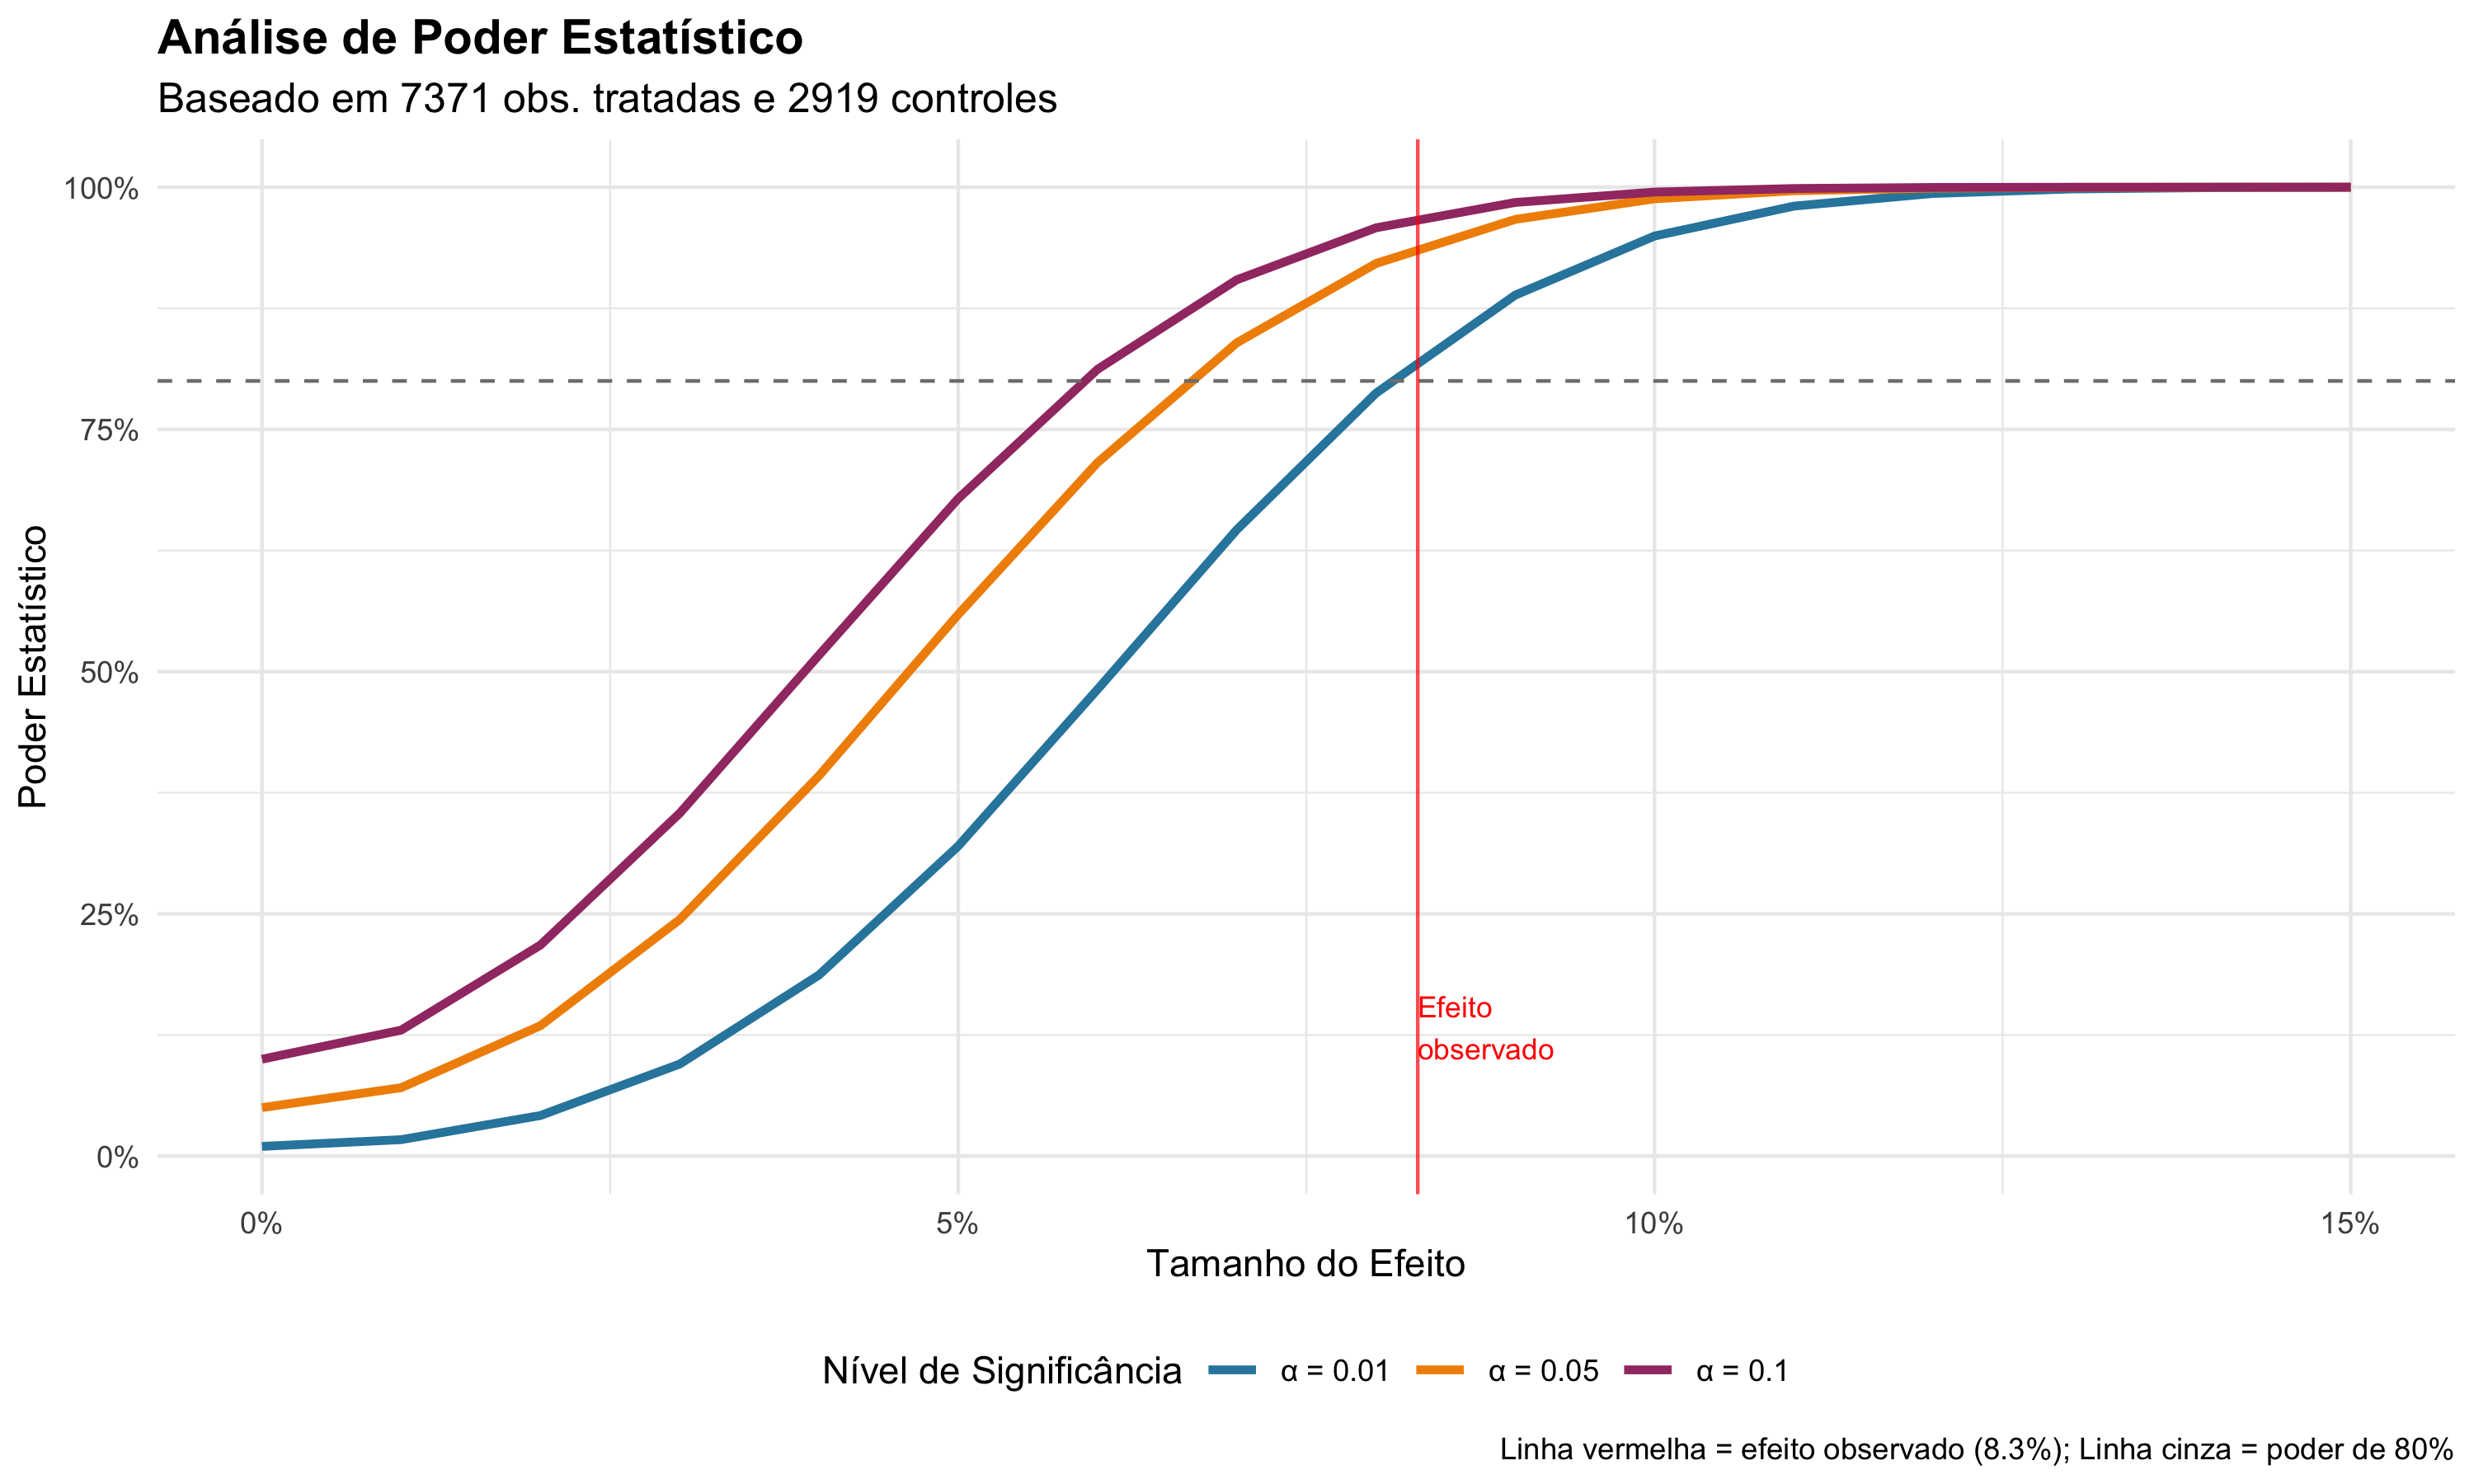
\includegraphics[width=0.75\textwidth]{../../../data/outputs/additional_figures/power_analysis_simulation.png}
\end{figure}

\begin{itemize}
    \item Para o efeito de 8,2\%: poder de 92,1\% ($\alpha$ = 0,05)
    \item Design adequado para detectar efeitos economicamente relevantes
    \item Mínimo efeito detectável com 80\% de poder: ~5,5\%
\end{itemize}
\end{frame}

\begin{frame}{Backup: Processo de Integração dos Dados}
\begin{columns}
\column{0.5\textwidth}
\textbf{Fontes de Dados:}
\begin{itemize}
    \item \textbf{INMET}: 610 estações meteorológicas
    \item \textbf{IBGE}: PIB municipal e população  
    \item \textbf{PAM-IBGE}: Produção agrícola detalhada
\end{itemize}

\textbf{Plataforma de Integração:}
\begin{itemize}
    \item Google BigQuery + basedosdados
    \item Acesso unificado às bases públicas
    \item SQL otimizado para grandes volumes
\end{itemize}

\column{0.5\textwidth}
\textbf{Pipeline de Processamento:}
\begin{enumerate}
    \item Extração via API Python
    \item Agregação município → microrregião
    \item Validação cruzada de mapeamentos
    \item Tratamento de dados faltantes
    \item Construção do painel balanceado
\end{enumerate}

\begin{block}{Dataset Final}
490 microrregiões × 21 anos = 10.290 obs\\
0\% de valores faltantes
\end{block}
\end{columns}
\end{frame}

\begin{frame}{Backup: Heterogeneidade Regional}
\begin{table}[h]
\centering
\begin{tabular}{lccc}
\toprule
Região & ATT & EP & N Tratadas \\
\midrule
Norte & 0,095 & (0,041) & 8 \\
Nordeste & 0,076** & (0,035) & 45 \\
Centro-Oeste & 0,091*** & (0,028) & 22 \\
Sudeste & 0,083*** & (0,024) & 48 \\
Sul & 0,089** & (0,038) & 8 \\
\bottomrule
\end{tabular}
\end{table}

\begin{itemize}
    \item Efeitos positivos em todas as regiões
    \item Magnitude similar (7,6\% a 9,5\%)
    \item Maior precisão em regiões com mais observações
    \item Sugere validade externa dos resultados
\end{itemize}
\end{frame}

\begin{frame}{Backup: Detalhes da Implementação Computacional}
\begin{columns}
\column{0.5\textwidth}
\textbf{Software e Pacotes:}
\begin{itemize}
    \item R 4.5.0 + pacote \texttt{did} v2.1.2
    \item Python 3.11 + \texttt{basedosdados}
    \item Google BigQuery API
    \item Sistema \texttt{renv} para reprodutibilidade
\end{itemize}

\textbf{Especificações Técnicas:}
\begin{itemize}
    \item Bootstrap: 1.000 replicações
    \item Clustering: nível microrregião
    \item Inferência: bandas uniformes
\end{itemize}

\column{0.5\textwidth}
\textbf{Escolhas Metodológicas:}
\begin{itemize}
    \item Estimador: Doubly Robust
    \item Controle: not-yet-treated
    \item Covariáveis: pré-tratamento
    \item Agregação: balanceada (event study)
\end{itemize}

\textbf{Validações:}
\begin{itemize}
    \item Convergência do bootstrap
    \item Estabilidade numérica
    \item Sensibilidade a outliers
\end{itemize}
\end{columns}
\end{frame}

\end{document}
